\section{Method}
\label{sec:method}

In this section our approach to solve the Automatic Lip-reading is presented.
The high-level architecture is first introduced, where the main components and their functions is described.
The particular architectures which we like to evaluate is then presented.

\subsection{Single-View Lip-Reading}

\subsubsection{Bi-directional LSTM}
We consider the directional sequence with applying bi-directional LSTM. We put the backward LSTM layer on the output of the forward LSTM. Now we can consider the history of the previous and next data.



\subsubsection{Batch Normalization}
We additionally put Batch Nromalization layer on the output of the LSTM or bi-LSTM. Unlike BN after CNN, normalization is done on feature-wise method, which is each feature map in the input will be normalized separately, but using per-batch statistics to normalize the data during both testing and training.

\subsection{Multi-View Lip-Reading}
In Multi-view, we similarly applied bi-LSTM and Batch Normalization. Beside, there is several different architecture of visual model to get input of five views. Here, we introduce four architecture of visual model. 
\subsubsection{Visual Model Architecture}
\begin{figure}[h]
	\centering
	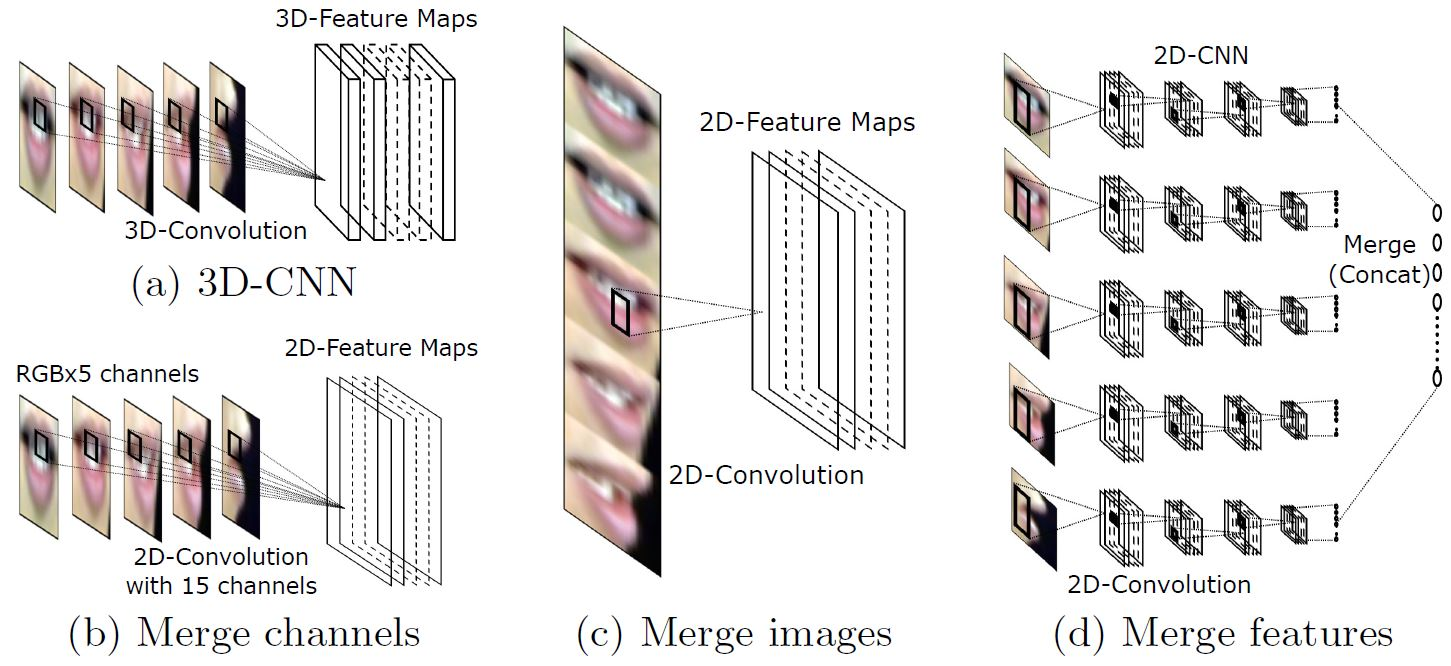
\includegraphics[width=\columnwidth]{fig/multi.jpg}
	\caption{Various visual model suggestions for the multi-view setting}
	\label{fig:multi}
\end{figure}
\begin{itemize}
	\item \textbf{3D-CNN}
	We construct 3D-CNN as almost same as 2D-CNN, the filter shapes are
	(1,3,3) and (2,3,3) for the first and the second convolutional layer respectively as shown in Fig.\ref{fig:multi} (a). The shape of pooling size is (1,2,2) for every max-pooling layer, and the remaining parameters are same as 2D-CNN. Strictly speaking, the five view data is not a 3-dimensional data. However, we conduct an experiment with 3D-CNN to find out the possibilities of learning some features or not.
	\item \textbf{Merge Channels}
	We make an input image having 15 channels from the five view data with three (RGB) channels as shown in Fig.4. (b). The places in the same pixel position of each view data are the different locations in actual. Although it looks somewhat weird, we conduct this experiment as the same reason as 3D-CNN.
	\item \textbf{Merge Images}
	As shown in Fig.4. (c), we append five images from the different view at the same time into a single image as an input of the visual model. In this architecture, we expect to learn all the five view feature by 2D-CNN. While out of our experiment, a more elaborate configuration is that all five images avoid convolving each other along the edges.
	\item \textbf{Merge Features}
	The last variation is shown in Fig.4. (d). We merge the fea- tures that are generated by 2D-CNN from the images in the different view at the same time. We design this architecture to learn each view image separately and to combine them into a single feature for an input of the temporal model.
\end{itemize}
\subsubsection{Data-Augmentation}
In deep learning approach, the most important thing is the amount of the data. With much data, we can learn it more easier with better performance. Thus there are some method for augmenting the given data. We apply the simple data augmentation for our given data set. In our training set, there are 5 types of views(view 1,2,3,4,5). And view 2,3 and 3,4 are very similar.  So we can augment the data with substitution view 2,3 and view 3,4. With the data augmentation, we trained with 5 times of amount of given data.

%
%\subsection{High-level Architecture}
%In figure \ref{fig:highLevelArchitecture} an illustration of the high-level architecture can be seen with the three main components; \textit{Visual model}, \textit{temporal model} and classifier.
%In the figure the flow of information can also be seen, from the sequence of images inputted to the architecture and to the outputted class probabilities. 
%%For this project the \textit{input} data consist of a sequence of images, where the dataset presented in section \ref{sec:dataset} is used the extracted region-of-interest.
%The \textit{visual model} is used to extract features from the input image.
%These features is then passed on to the \textit{temporal model} where they are correlated in time.
%The time correlated features is then inputted to the classifier which is outputting the different class probabilities.
%For each of the three main components, different implementations is of interest where each of these is listed in figure \ref{fig:highLevelArchitecture}. 
%Each of the different methods is presented in the following sections.
%We would here evaluate the performance where a single method from each component is used in combination, which give a total of 16 different architectures.
%\begin{figure}[h]
%    \centering
%    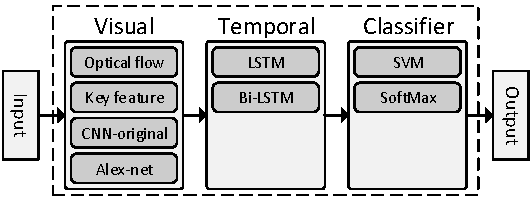
\includegraphics[width=\columnwidth]{fig/highLevelArchitecture.pdf}
%    \caption{High-level architecture used in this work, with the three main component and with the different method used for each of them.}
%    \label{fig:highLevelArchitecture}
%\end{figure}
%
%\subsection{Visual Model}
%For the feature extraction 4 different methods is of interest, where two of these make use of neural network's and the other two is computer vision related.
%\paragraph{CNN-original}
%This visual model is corresponding to the one used in the state-of-the-art model, presented in \cite{Lee}.
%An illustration of the model can be seen in figure \ref{fig:cnnOriginal}.
%It make use of two convolutional layers with 16 to 256 filters in the shape of (3,3).
%Each convolutional layer has a successive max-pooling layer in the shape of (2,2).
%Lastly a fully connected layer with a dimension of 8 to 64 outputs is used.
%\begin{figure}[h]
%    \centering
%    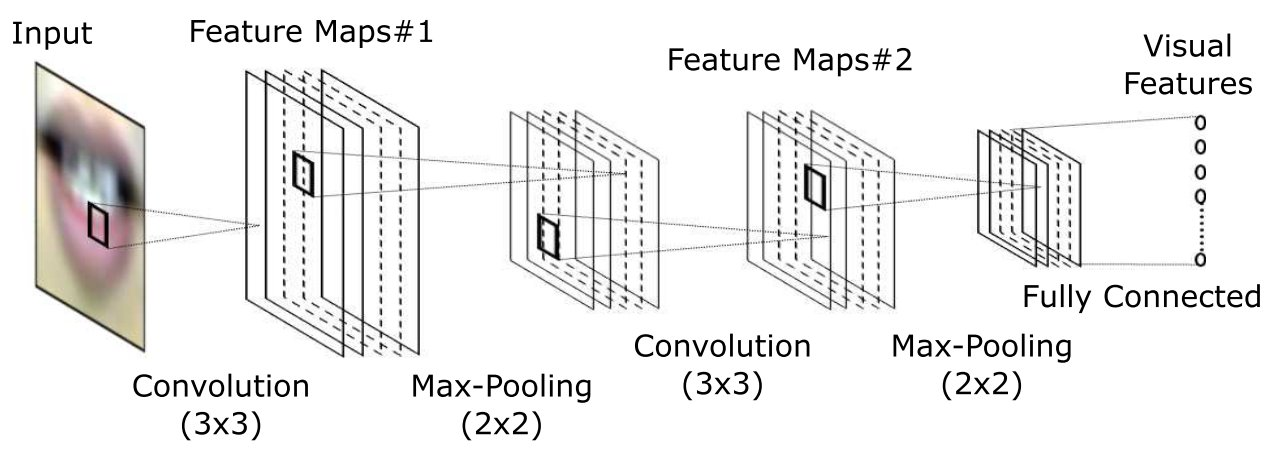
\includegraphics[width=\columnwidth]{fig/cnnOriginal.jpg}
%    \caption{CNN-original\cite{Lee}}
%    \label{fig:cnnOriginal}
%\end{figure}
%
%\paragraph{Alex-Net}
%A popular neural network architecture for image recognition is an Alex-net\cite{Krizhevsky2012}.
%This architecture is a deep CNN as depicted in figure \ref{fig:alexNet}.
%\begin{figure}[h]
%    \centering
%    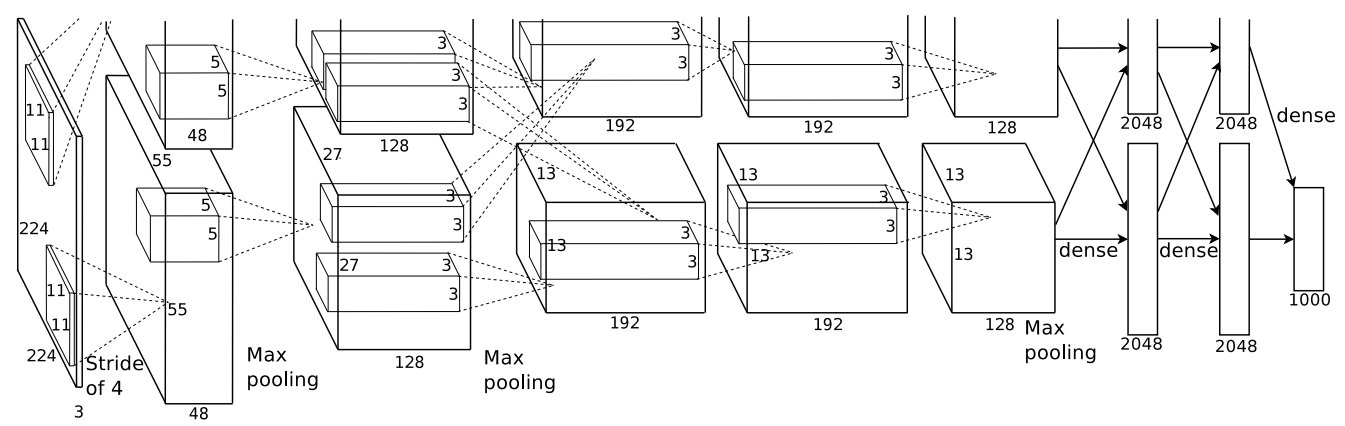
\includegraphics[width=\columnwidth]{fig/alexNet.jpg}
%    \caption{Alex-net\cite{Krizhevsky2012}}
%    \label{fig:alexNet}
%\end{figure}
%
%\paragraph{Optical flow}
%For the calculation of optical flow we expect the differential method commonly denoted as the Lucas-Kanade method\cite{Lucas1981}.
%The method have the assumption of the flow begin essentially constant in a local neighbourhood.
%
%\paragraph{Key features}
%For the key feature extraction a method similar to the one presented in \cite{Li2008} is used.
%The mouth is divided in to four parts, lower and upper part of the upper lip and lower and upper part of the lower lip.
%A vertical grid is then made, where the coordinates of the intersection points is used.
%An illustration of this can be seen in figure \ref{fig:keyFeature}.
%\begin{figure}[h]
%    \centering
%    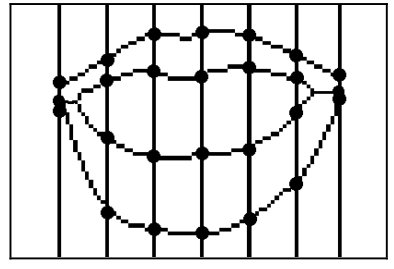
\includegraphics[width=0.5\columnwidth]{fig/keyFeature.jpg}
%    \caption{Key Feature\cite{Li2008}}
%    \label{fig:keyFeature}
%\end{figure}
%
%\subsection{Temporal model}
%Two different temporal models is used, which is \textit{LSTM} and \textit{bidirectional-LSTM}.
%For both of these models a two layered design is used, where the size of each layer is here varying with the number of output features from the visual model.
%
%\subsection{Classifier}
%There are many kinds of classifier to determine the output. In our approach, we will apply two different classifier, namely a support vector machine (SVM) and softmax function. SVM classify the data points with some vectors that can divide whether correct or not. Softmax function normalizes the probabilities and reconstruct it with distinct difference.

%\subsection{Proposed Architecture}
%We propose to use several different model for both the visual and temporal model.
%We will here implement and evaluate each of these models to see how they perform and compare this to the current state-of-the-art architecture.
%We will here use the visual and temporal models listed in table \ref{tab:visualTemporalModel}.

%\begin{table}
%\centering
%\begin{tabular}{l|l}
%Visual Model & Temporal Model\\
%\hline
%CNN-original & LSTM\\
%Alex-net & B-LSTM\\
%Optical Flow & \\
%Key Features &
%\end{tabular}
%\caption{Table with the different Visual and Temporal models used}
%\label{tab:visualTemporalModel}
%\end{table}

%From these visual and temporal models a total of 10 different architectures can be obtained by combining a single visual model with a single temporal model.
%These 10 single model architectures is all listed in table \ref{tab:singleModelArc}.
%Beside these single model architecture further can be obtained by combining multiple visual models with a single temporal model.
%Before combining multiple visual models, we first propose to evaluate the performance of the single model architectures.
%
%
%In our approach we will first obtain results from the 10 basic models and then 
%
%
%Temporal Model
%LSTM
%B-LSTM
%
%
%Alex-net + LSTM
%CNN-original + Bidirectional LSTM
%Optical flow + LSTM
%Key features + LSTM
